\subsection{Datenvorverarbeitung}
\label{subsec:Datenvorverarbeitung}
Nach der Datenbeschaffung erfolgt die Datenvorverarbeitung, die darauf abzielt, die Qualität und Integrität der Daten sicherzustellen. Ein zentraler Schwerpunkt liegt dabei auf der Identifikation und Eliminierung fehlerhafter oder ungültiger Datensätze. Häufig wird innerhalb der Datensätze nach Nullwerten gesucht, um diese entweder durch valide Daten zu ersetzen oder in einigen Fällen gänzlich zu entfernen. Im vorliegenden Fall ist es wichtig, dass sämtliche als verwendbar gekennzeichneten Hotels in die Analyse einbezogen werden. Die Datensätze sollen nicht einfach verworfen werden; vielmehr erfolgt eine gezielte Substitution von Nullwerten durch valide Daten, um eine konsistente und zuverlässige Grundlage für die weiterführende Analyse zu gewährleisten \cite{Agarwal.05.10.2018}.
\newline
\newline
Im Folgenden ist die Anzahl aller Nullwerte innerhalb des Datensatzes zu sehen:
\begin{figure}[h]
    \centering
    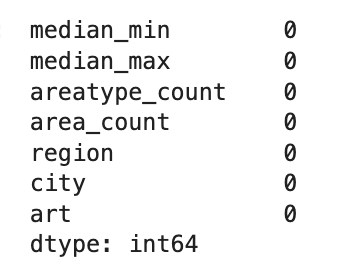
\includegraphics[width=0.4\textwidth, center]{Null_values.png}
    \caption[Summe aller Nullwerte im Datensatz]{Summe aller Nullwerte im Datensatz}
    \label{img:null_values}
\end{figure}

In Abbildung \ref{img:null_values} ist zu sehen, dass innerhalb des es Datensatzes keine Nullwerte gibt und somit auch keine Datenvorverarbeitung getätigt werden muss.